\chapter{Аналитическая часть}
\section{Инфиксная и постфиксная нотация}
Инфиксная нотация -- это стандартная форма записи математических выражений, в которой операторы располагаются между операндами. Например, выражение \texttt{A + B} представляет операцию сложения двух переменных A и B. Инфиксная нотация требует явного указания порядка операций с использованием скобок.

Это форма записи математических выражений, где операторы следуют за операндами. Например, выражение \texttt{A B +} в постфиксной нотации также представляет операцию сложения. Эта форма не требует скобок для определения порядка операций, что упрощает процесс вычисления.
\section{Преимущество постфиксной нотации}
Главное преимущество постфиксной нотации (обратной польской записи) заключается в том, что при её разборе нет необходимости расставления скобок и в связи с этим такую запись легко представить в виде бинарного дерева, а следовательно и составить компьютерный алгоритм. Рассмотрим, на рисунке \ref{fig:2}, пример: 1,2,+,2,3,*,/.
\begin{center}
	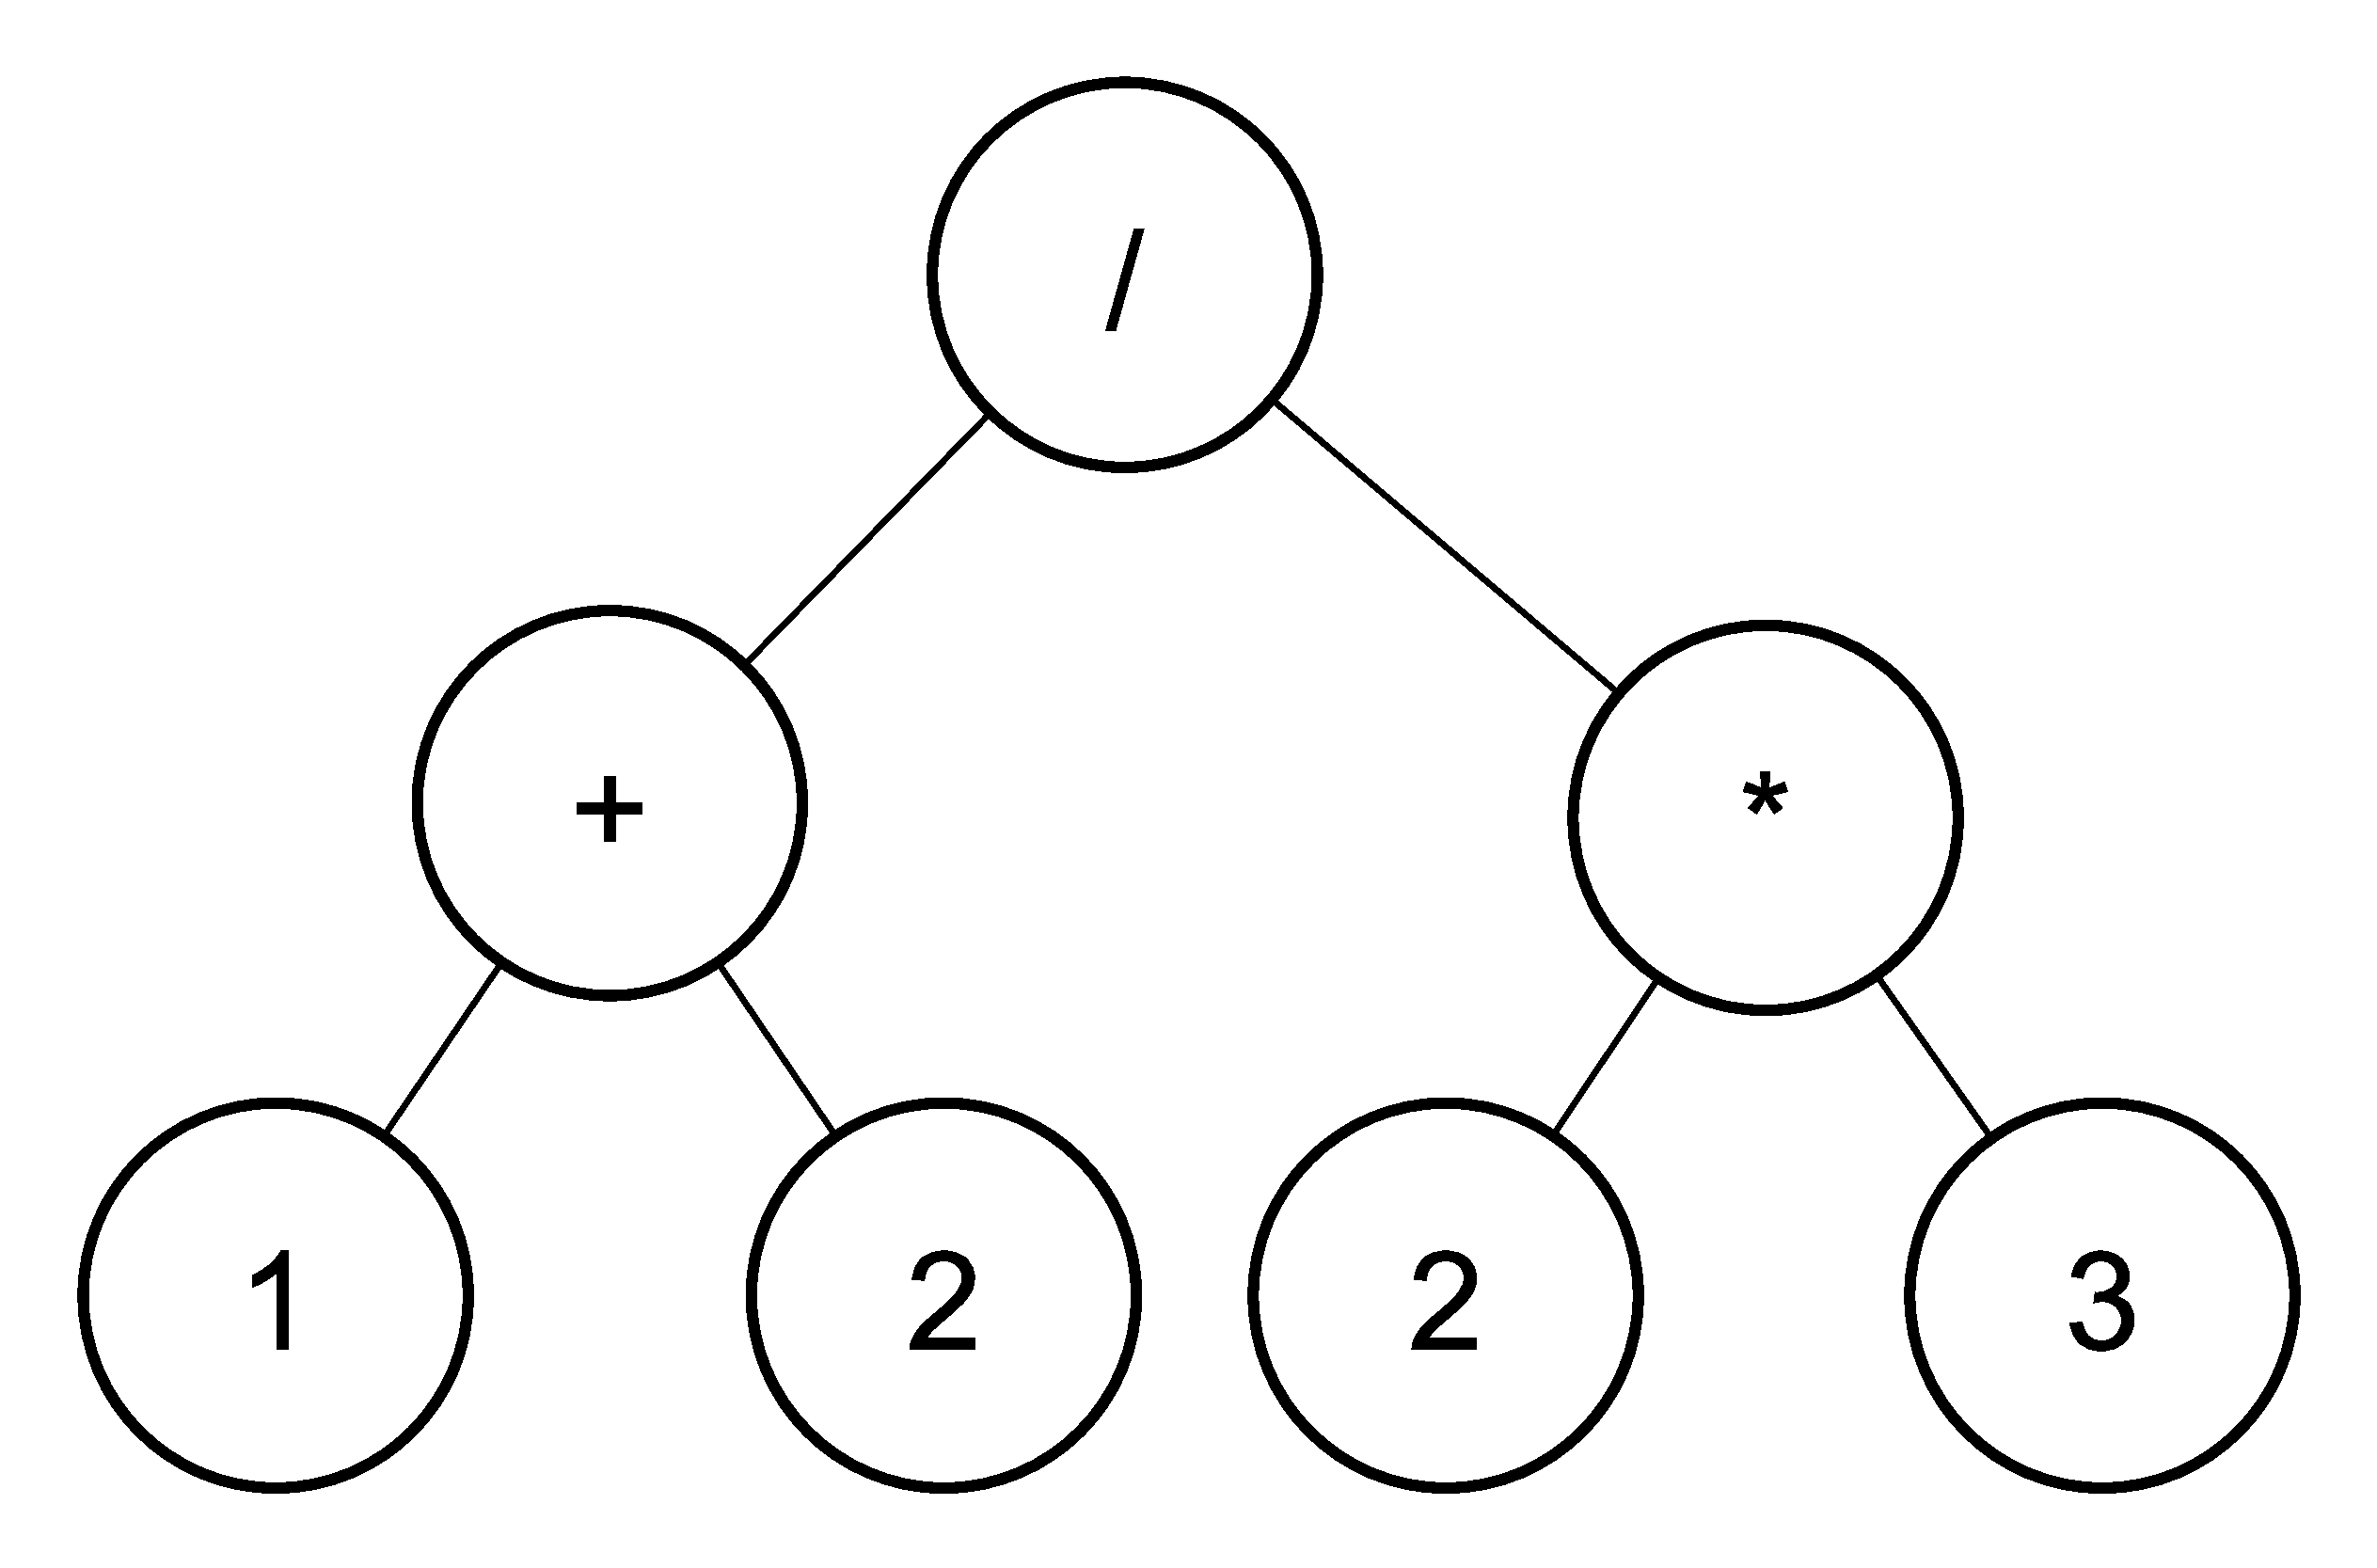
\includegraphics[width = 15cm]{bin_tree}
	\captionof{figure}{Дерево постфиксной записи}
	\label{fig:2}
\end{center}
\clearpage
